\subsection{Besonderheiten der FM-Synthese}
\FloatBarrier
\subsubsection{Zusammenhang zwischen Phasen- und Frequenzmodulation}
Frequenzmodulation (FM) und Phasenmodulation (PM) können unter dem Oberbegriff Winkelmodulation zusammen gefasst werden. Im Folgenden soll der Zusammenhang zwischen PM und FM genauer beschrieben werden. Zuerst wird die mathematische Herleitung der beiden Modulationen beschrieben. Anschließend wird die Ähnlichkeit der beiden Verfahren erörtert und im Kontext der Akustik beschrieben.
Interessanterweise führte die Publikation von Chowning zu anfänglicher Verwirrung. In seinem Artikel definiert er eine Formel, welche einer PM gleicht. Zusätzlich beschreibt er ein MUSIC~V Patch der eine FM implementiert. Beides wird jedoch von ihm als FM-Synthese vorgestellt. \cite{rossum1999method} Des Weiteren kann dem Yamaha Patent für die Implementierung eines FM-Synthesizer entnommen werden, dass Yamaha ihre FM-Synthese über eine Phasenmodulation erzeugte. \cite{oya1987electronic} 

Wie der Name Winkelmodulation andeutet, wird der Phasenwinkel eines Trägersignals in Abhängigkeit eines Modulationssignals verändert. Die Amplitude \(A\) bleibt während der Modulation konstant. In der allgemeinsten Form kann ein winkelmoduliertes Signal als Sinusfunktion eines sich zeitlich ändernden Winkels beschrieben werden:
\begin{equation}
s(t)=A\cdot\sin(\theta(t))
\label{eq:signal_basis_funktion}
\end{equation}
Dabei wird \(\theta(t)\) als \textit{momentaner Phasenwinkel} bezeichnet und ist als Summe der konstanten Kreisfrequenz $\omega_0$ multipliziert mit der Zeit $t$ und der \textit{momentanen Phasenverschiebung} $\varphi(t)$ definiert:
\begin{equation*}
\theta(t)=\omega_0t + \varphi(t)
\end{equation*}
Ein Großteil der Frequenzen in diesem Kapitel beziehen sich auf eine Schwingung, welche selbst auf eine Kreisbewegung zurückgeführt werden kann. Daher macht es Sinn Frequenzen $f$ als Kreisfrequenz $\omega$ anzugeben. Zwischen Frequenz und Kreisfrequenz gilt $\omega=2\pi f$.


Wird nun die momentane \textbf{Phasenverschiebung} des Trägersignals proportional zum Modulationssignal \(p(t)\) verändert, erhält man das \textbf{phasenmodulierte} Signal \(s_{PM}(t)\). \cite[S. 209]{lathi}
Für die momentane Phasenverschiebung ergibt sich folgende einfache Formel:
\begin{equation}
\varphi(t)=\varphi_0+k_{PM}\cdot p(t)
\label{eq:varphi_t}
\end{equation}
Für akustische Anwendungen wird der konstante Teil \(\varphi_0\) der Phasenverschiebung nicht benötigt und wird, ohne Beschränkung der Allgemeinheit, als Null angenommen.
Bei \(k_{PM}\) handelt es sich um eine Proportionalitätskonstante, welche Modulatorkonstante genannt wird. Die Modulatorkonstante bestimmt, wie stark das Modulationssignal auf das Trägersignal einwirkt. Wird nun \(\theta(t)\) in die allgemeine Formel~\ref{eq:signal_basis_funktion} für ein moduliertes Signal substituiert und das obige \(\varphi(t)\) eingesetzt, ergibt sich die Formel für das phasenmodulierte Signal:
\begin{equation}
s_{PM}(t)=A\cdot\sin(\omega_0t + \varphi(t))=A\cdot\sin(\omega_0t+k_{PM}\cdot p(t))
\label{eq:s_pm}
\end{equation}
Für die Herleitung der Frequenzmodulation muss zuvor noch der Begriff der \textit{momentanen Kreisfrequenz} \(\omega(t)\) eingeführt werden.
Diese entspricht der Änderung des Phasenwinkels in Abhängigkeit der Zeit. Daher kann die momentane Kreisfrequenz durch die erste Ableitung des Phasenwinkels nach der Zeit $\dot \theta(t)$ bestimmt werden. \cite[S. 209]{lathi}
\begin{equation}
\omega(t)=\dot \theta(t)=\frac{d\theta(t)}{dt}=\frac{d[\omega_0t+\varphi(t)]}{dt}=\frac{d\omega_0t}{dt}+\frac{d\varphi(t)}{dt}=\omega_0+\frac{d\varphi(t)}{dt}
\label{eq:omega_m_herleitung}
\end{equation}
Wieso dieser Zusammenhang gültig ist, lässt sich einfach veranschaulichen. Bei \(\omega\) handelt es sich um die Kreisfrequenz, also wie häufig eine Schwingung einen Kreis pro Zeitspanne durchläuft, hier in Sekunden. Bei einer Kreisfrequenz von \(\omega=2 s^{-1}\) wird ein Phasenwinkel von \(4\pi\) pro Sekunde überstrichen. Wird nun die Kreisfrequenz erhöht, wird ein größerer Phasenwinkel überstrichen. Daher gibt die momentane Kreisfrequenz die Änderungsrate des momentanen Phasenwinkels zu einem bestimmten Zeitpunkt \(t\) an. Da die Änderung einer Funktion der Ableitung dieser Funktion entspricht, ergibt sich der Zusammenhang aus der obigen Formel. 
Eine Analogie aus der Physik hierzu ist, der Zusammenhang zwischen dem Weg \(s(t)\) und der Geschwindigkeit \(v(t)\). Die Geschwindigkeit gibt die Änderung des Weges pro Zeiteinheit vor. Somit gilt \(\dot{s(t)}=v(t)\). In unserem Zusammenhang verhält sich die Kreisfrequenz analog zur Geschwindigkeit und der Phasenwinkel ist im Prinzip die Strecke ausgedrückt als Winkel.

Wird die momentane \textbf{Frequenz} des Trägersignals proportional zum Modulationssignal \(f(t)\) verändert, erhält man das \textbf{frequenzmodulierte} Signal \(s_{FM}(t)\). \cite[S. 210]{lathi} Für die momentane Frequenz ergibt sich analog zur Phasenmodulation folgende Formel:
\begin{equation}
\omega(t)=\omega_0+k_{FM}\cdot f(t)
\label{eq:omega_m}
\end{equation}

Bei \(k_{FM}\) handelt es sich wieder um eine Modulatorkonstante. Sie gibt an wie stark das Modulationssignal das Trägersignal beeinflusst. Um nun das frequenzmodulierte Signal zu erhalten muss die momentane Frequenz, analog wie bei der Phasenmodulation, in \(s(t)\) eingesetzt werden. Jedoch kommt \(\omega(t)\) nicht direkt in \(s(t)\) oder \(\theta(t)\) vor. Aus Formel~\ref{eq:omega_m_herleitung} ist bekannt, dass die momentane Frequenz gleich der ersten Ableitung des momentanen Winkels \(\theta(t)\) ist. Im Umkehrschluss bedeutet das, dass die Integration von \(\omega(t)\) nach der Zeit gleich \(\theta(t)\) sein muss.
\begin{equation*}
\theta(t)=\int_0^t{\omega(\tau)} d\tau = \int_0^t{\omega_0 + k_{FM}\cdot f(\tau)} d\tau = \omega_0t + k_{FM} \cdot \int_0^t{f(\tau)} d\tau
\end{equation*}
Wird dieser Term in $s(t)$ eingesetzt, ergibt sich die Formel für ein frequenzmoduliertes Signal:
\begin{equation}
s_{FM}(t)=A\cdot\sin(\omega_0t + k_{FM} \cdot \int_0^t{f(\tau)} d\tau)
\label{eq:s_fm}
\end{equation}
Es sei angemerkt, dass wissentlich die Integrationskonstante mit Null gleichgesetzt wurde und somit nicht in den Formeln auftritt, da sie für unsere Beobachtungen unerheblich ist und die Terme nur unnötig verkomplizieren würde.

Wie einführlich erklärt, ist die Phasenmodulation mit der Frequenzmodulation verwandt. Wie ähnlich die beiden Verfahren sind, ist leicht an den Formeln für die modulierten Signalen~\ref{eq:s_pm} und \ref{eq:s_fm} ersichtlich . Beide Formeln sind bis auf die letzte Addition gleich. Daraus lässt sich eine Bedingung ableiten, welche beschreibt wann eine FM durch eine PM oder umgekehrt dargestellt werden kann. Dies ist genau dann möglich, wenn die Signale \(s_{PM}(t)\) und \(s_{FM}(t)\) identisch sind. Daraus ergibt sich für die Modulationssignale \(p(t)\) und \(f(t)\) folgende Beziehung:
\begin{equation}
k_{PM}\cdot p(t)=k_{FM} \cdot  \int_0^t{f(\tau)} d\tau
\end{equation}

Vorausgesetzt \(k_{PM}\) ist gleich \(k_{FM}\), dann können beide Faktoren aus der Gleichung eliminiert werden. Ist es nun möglich, für \(f(t)\) eine Ableitung zu finden, kann eine PM durch eine FM dargestellt werden. Durch die Ableitung von \(\int_0^t{f(\tau)}d\tau\) wird das Integral aufgehoben und die Gleichung reduziert sich zu einem einfachen \(p(t)=f(t)\). Umgekehrt gilt, dass genau dann eine FM durch eine PM dargestellt werden kann, wenn \(p(t)\) integrierbar ist. Unter diesen Bedingungen sind beide Verfahren, mathematisch betrachtet, gleich. Daher kann nur anhand der Betrachtung eines modulierten Signals nicht darauf zurück geschlossen werden, ob es mit einer Phasen- oder Frequenzmodulation erzeugt wurde. Die unterschiedlichen Namen (FM, PM) zeigen somit nur, welche Größe des Modulationssignals (\(f(t), p(t)\)) proportional ist. \cite[S. 210]{lathi}

Eine weitere, erwähnenswerte Eigenschaft lässt sich gewinnen, wenn die momentane Phasenverschiebung beider Verfahren gegenüber gestellt wird. Während \(\varphi(t)\) für PM durch die Formel~\ref{eq:varphi_t} gegeben ist, muss \(\varphi(t)\) für FM durch gleichsetzten der Formeln~\ref{eq:omega_m_herleitung} und \ref{eq:omega_m} gewonnen werden:
\begin{eqnarray*}
\omega_0+\frac{d\varphi(t)}{dt}&=&\omega_0+k_{FM}\cdot f(t) \\
\frac{d\varphi(t)}{dt}&=&k_{FM}\cdot f(t)
\end{eqnarray*}
Daraus ergibt sich für ein gemeinsames Modulationssignal \(m(t)\) folgender Zusammenhang:
\begin{center}
\fbox{\parbox{7.5cm} { 
	\begin{eqnarray*}
	\varphi(t)&=&k_{PM}\cdot m(t) : \textbf{PM} \\
	\frac{d\varphi(t)}{dt}&=&k_{FM}\cdot m(t) : \textbf{FM}
	\end{eqnarray*}
}}
\end{center}
Da $\frac{d\varphi(t)}{dt}$ die Ableitung und somit die Änderung von $\varphi(t)$ ist, ändert sich $\varphi(t)$ wenn die Ableitung sich ändert und umgekehrt. PM und FM treten also immer gleichzeitig auf.
% [TODO cite lathi?]

Bisher wurde nur das modulierte Signal betrachtet und dessen Abhängigkeit von den allgemeinen Modulationssignalen \(p(t)\) bzw. \(f(t)\). Für die bisherigen Erkenntnisse war es einfach nicht notwendig, sich auf spezifische Modulationssignale festzulegen. Diese allgemeine Betrachtung ist jedoch mehr für die Nachrichtentechnik, als für einen FM-Synthesizer interessant.
Daher werden die folgenden Formeln im Kontext der Akustik betrachtet und weniger streng mathematisch, wie bisher. So kann zum Beispiel das menschliche Gehör keine initiale Phasenverschiebungen wahrnehmen. Dies erlaubt Umformungen von Termen, die mathematisch nicht korrekt sind, jedoch am Ergebnis, also dem hörbaren Klang, keine Auswirkung haben. Deshalb ist es korrekt, bei den obigen Umformungen den initialen Phasenwinkel $\varphi_0$ zu ignorieren. Des Weiteren wird im Folgenden ein sinusförmiges Signal als Modulator verwendet, welches sowohl für die PM als auch für die FM verwendet wird und wie folgt definiert ist:
\begin{equation}
m(t)=f(t)=p(t)=\sin(\omega_m t)
\end{equation}
Wobei \(\omega_m\) die Modulationskreisfrequenz darstellt. Eingesetzt in die Formeln für PM und FM ergibt sich:
\begin{eqnarray*}
s_{PM}(t)&=&A\cdot\sin(\omega_0t+k_{PM}\cdot\sin(\omega_m t)) \\
s_{FM}(t)&=&A\cdot\sin(\omega_0t+k_{FM}\cdot\int_0^t{\sin(\omega_m \tau)} d\tau)
\end{eqnarray*}
Die von Chowning vorgestellte Formel gleicht der Formel für eine PM, \cite{chowningPaper} wobei Chowning seine Formel als Frequenzmodulation vorstellt. Wieso diese Aussage trotzdem korrekt ist, wird im Folgenden gezeigt. Im ersten Schritt muss das Integral innerhalb von \(s_{FM}(t)\) ausgerechnet werden:
\begin{equation*}
s_{FM}(t)=A\cdot\sin(\omega_0t-\frac{k_{FM}}{\omega_m}\cdot\cos(\omega_m t))
\end{equation*}
Mathematisch gesehen unterscheidet sich diese Formel zu einer Phasenmodulation. Genauer gesagt ergibt die Integration eine Verschiebung von $\frac{\pi}{2}$, da ein negativer Kosinus genau eine viertel Periode phasenverschoben zu einem Sinus ist. Wie bereits erwähnt, nimmt das Gehör jedoch keine initiale Phasenverschiebungen wahr. Unter dieser Annahme, kann der negative Kosinus mit einem positiven Sinus ausgetauscht werden, ohne eine hörbare Veränderung des Tones zu erzeugen.
\begin{equation*}
e(t)=A\cdot\sin(\omega_0t+\frac{k_{FM}}{\omega_m}\cdot\sin(\omega_m t))
\end{equation*}
Die dadurch gewonnene Formel ähnelt in der Struktur der von Chowning vorgestellten Formel schon sehr. Jedoch ist in der obigen Formel der Modulationsindex $I$ nicht direkt ersichtlich. Dieser ist bei Chowning als $I=d/\beta$ definiert. Wobei $d$ dem Frequenzhub entspricht und $\beta$ der Modulationsfrequenz $\omega_m$ (s. Kapitel~\ref{chowningparameter}). Für den Frequenzhub $\Delta f$ gilt: \cite[S. 219]{lathi}
\begin{equation*}
\Delta f = k_{FM}\cdot [\dot f(t)]_{\max}
\end{equation*}
Da $f(t)$ eine Sinusfunktion darstellt, entspricht die Ableitung $\dot f(t)$ einer Kosinusfunktion und somit ist ihr Maximum gleich $1$ und entfällt in der obigen Formel. Somit reduziert sich der Frequenzhub zu $\Delta f=k_{FM}$ und kann in die obige Formel eingesetzt werden. Dadurch kann nun $\Delta f / \omega_m$ durch den Modulationsindex $I$ substituiert werden und es ergibt sich die originale Formel nach Chowning:
\begin{equation}
e(t)=A\cdot\sin(\omega_0t+I\cdot\sin(\omega_m t))
\label{eq:FM_Chowning}
\end{equation}
Diese Formel entspricht somit der von Chowning vorgestellten Formel für eine FM-Synthese und ist im Kontext der Akustik korrekt. Zusammengefasst wurde ersichtlich, dass die Formel von Chowning, streng mathematisch betrachtet, keine FM-Synthese darstellt, sondern eine \glqq PM-Synthese\grqq. Dieser feine Unterschied spielt jedoch in der Akustik kaum eine Rolle.
Im nächsten Kapitel werden Klangspektren berechnet um den Klangcharakter zu bestimmen. Um ein solches Klangspektrum zu bestimmen, muss bekannt sein welche Formel tatsächlich implementiert wurde.

\FloatBarrier
\subsubsection{Klangspektrum der FM-Synthese}
\label{bulli:ohrToeneUndFrequenzen}
Ein Ton wird durch eine einfache Sinusschwingung erzeugt. Die Lautstärke eines Tones, hängt von der Amplitude der Schwingung ab. Je größer die Amplitude desto lauter wirkt der Ton. Die Frequenz einer Schwingung empfindet der Mensch als Tonhöhe. Je größer die Frequenz desto höher wird der Ton empfunden. 
Das menschliche Ohr nimmt Frequenzen zwischen 16 Hz und 20 kHz wahr. Mit zunehmendem Alter nimmt die obere Hörschwelle ab. \cite[S. 199]{borucki}
Ein natürlicher Klang setzt sich nicht aus einer einzigen Frequenz zusammen, sondern aus mehreren Teiltönen. Jeder Teilton entspricht einem Sinuston mit einer bestimmten Frequenz, welche ein ganzzahliges Vielfaches des tiefsten Teiltones ist. Der tiefste Teilton, also der Teilton mit der niedrigsten Frequenz, wird als Grundton bezeichnet. \cite[S. 87]{borucki} 
Dabei kann das menschliche Gehör die Tonhöhe bestimmen, auch wenn der Grundton schwach ausgeprägt oder nicht vorhanden ist. \cite[S. 4]{zwicker} Abbildung~\ref{fig:geige} zeigt die Wellenform eines Geigentones und dem dazu gehörigen Frequenzspektrum.
Obwohl der Grundton wenig dominiert, die ersten acht Frequenzen sind in etwa gleichstark, würde das Ohr die Tonhöhe richtig erkennen.
Außerdem nehmen wir neben der Tonhöhe und Lautstärke eines Tones etwas Weiteres war. Das Spektrum eines Tones vermittelt uns ein Gefühl für unterschiedliche Klänge. Dieses Empfinden wird als Klangfarbe bezeichnet und lässt uns z.B. zwischen verschiedenen Instrumenten unterscheiden. \cite[S. 5]{zwicker} \cite[S. 226]{raichel}
Die stark vereinfachte Funktionsweise des menschlichen Ohrs, gibt Ausschluss darüber, warum Teiltöne entscheidend für den Klangcharakter sind. Die Schallwellen eines Klanges versetzten im Ohr, genauer in der Gehörschnecke, eine Flüssigkeit in Schwingung. Dadurch, dass die Gehörschnecke sich verengt, treffen die unterschiedlichen Frequenzen in Kombination mit der Amplitude, an unterschiedlichen Stellen auf Sinneshaare, welche die entsprechenden elektrischen Signale an das Gehirn weiterleiten. \cite[S. 87 f.]{zwicker}

\begin{figure} [ht]
\centering
  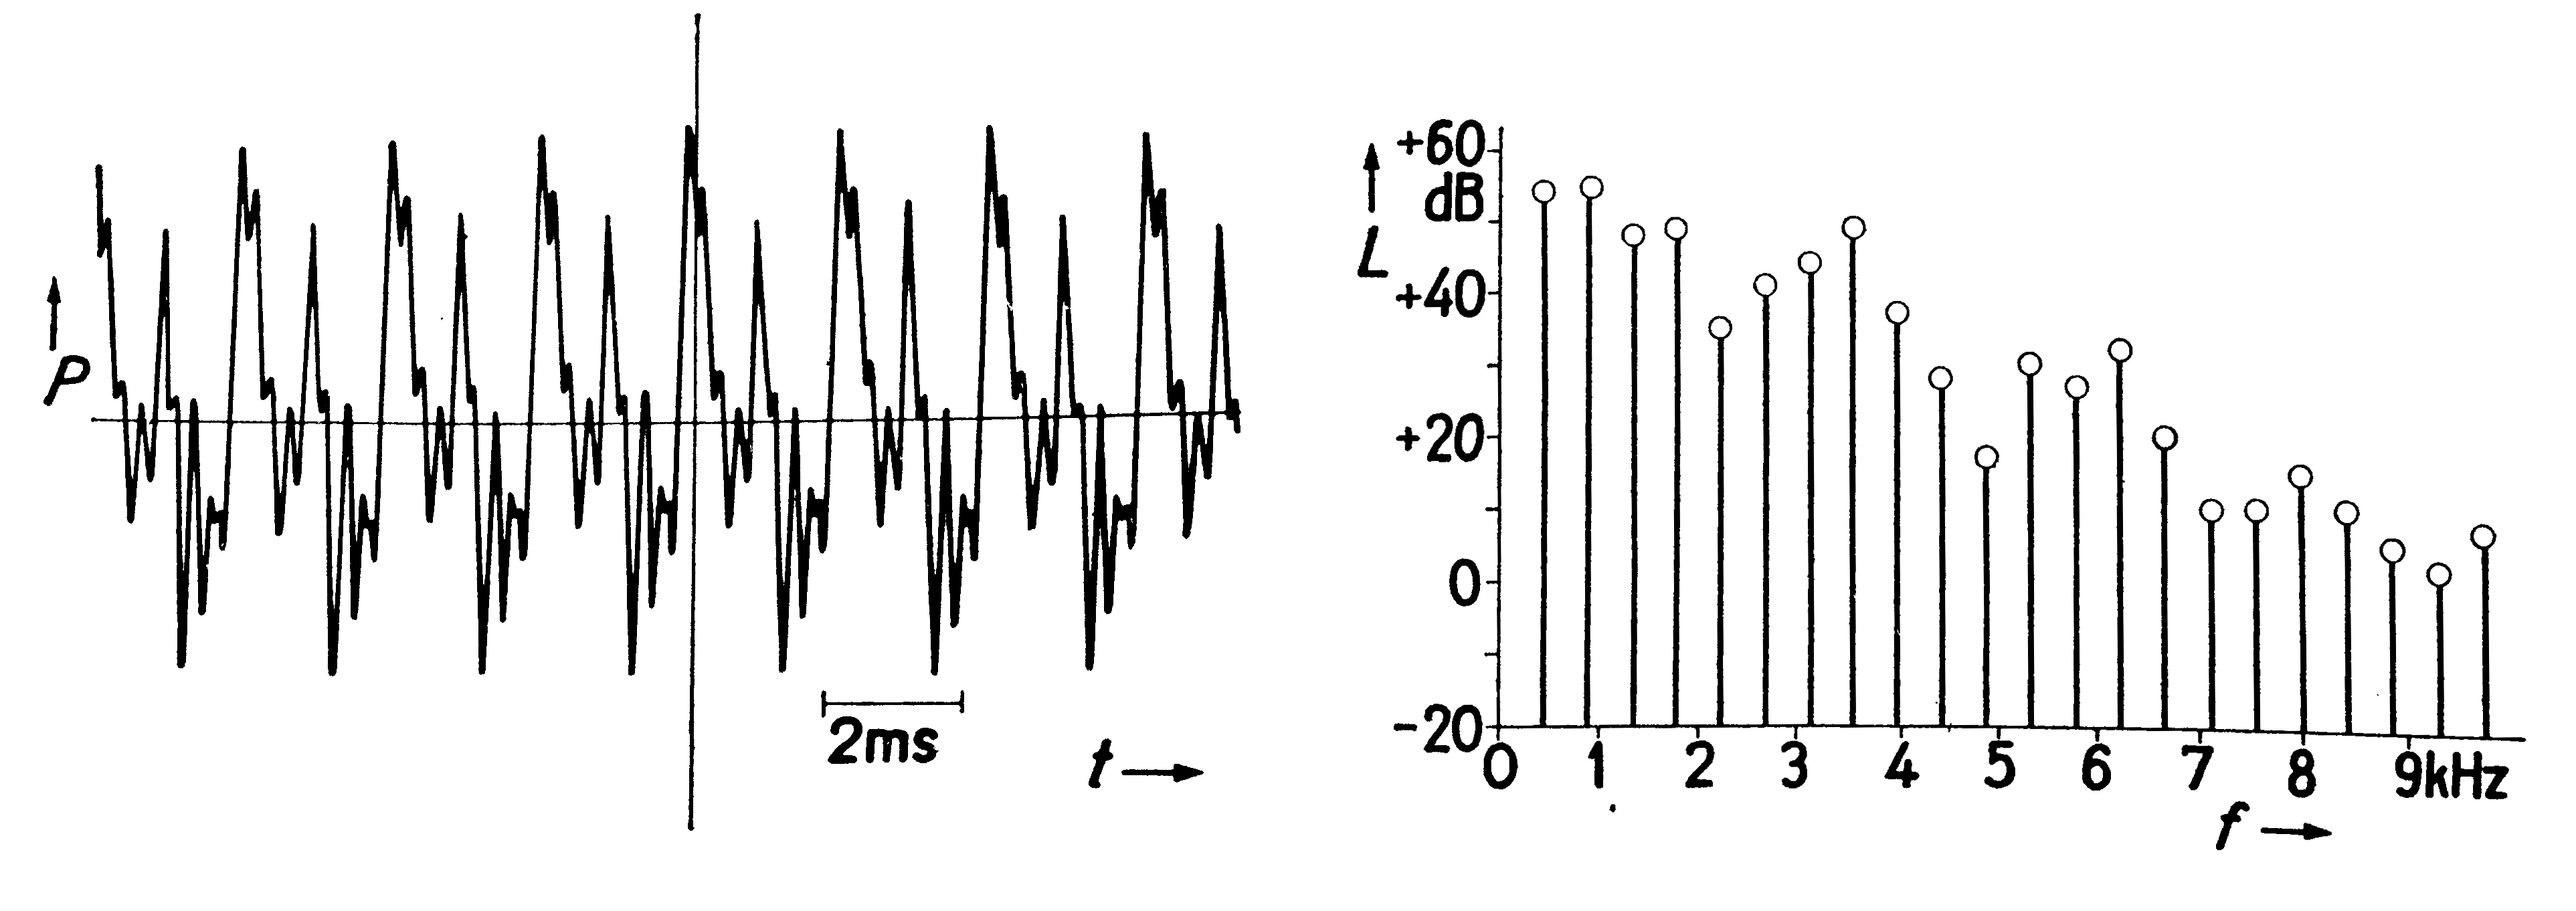
\includegraphics[width=0.95\textwidth]{GeigenTon.png}
\caption{Links: Schalldruck eines Geigenklangs; Rechts: Frequenzspektrum dieses Klanges}
\label{fig:geige}
Quelle: \cite[S. 4]{zwicker}
\end{figure}
\FloatBarrier

Bei der FM-Synthese treten Seitenschwingungen durch die zeitliche Änderung der Frequenz auf. Um daher einen ungefähren Eindruck eines synthetisierten Tones zu bekommen, reicht es nicht aus, die berechnete Kurve (Wellenform) zu betrachten, welche eine Funktion der Zeit ist. Daher muss eine alternative Darstellung des Signals gesucht werden. 
Hierzu eignet sich ein \textbf{Frequenzspektrum}. Es berechnet die Intensität einer gegeben Frequenz und ist somit eine Funktion der Frequenz. Das Frequenzspektrum lässt sich durch Fourier-Analyse bestimmen. So kann jede periodische, komplexe Sinuswelle als Fourier-Reihe dargestellt werden. Diese ist als Addition aus mehreren Teilsinuswellen mit unterschiedlichen Amplituden definiert. \cite[S. 33]{raichel} Durch mathematische Umformungen (siehe Kap.~\ref{matze:simplefm}) kann die Formel~\ref{eq:FM_Chowning} der FM-Synthese als folgende Summe dargestellt werden: \cite{chowningPaper}

\begin{equation}
\begin{split}
s(t)=A\cdot \{\; & J_0(I)\cdot\sin(\omega_c t)  \\
         +&J_1(I)\cdot [\sin(t\cdot (\omega_c + \;\,\omega_m))-\sin(t\cdot (\omega_c-\;\,\omega_m))] \\
         +&J_2(I)\cdot [\sin(t\cdot (\omega_c + 2\omega_m))+\sin(t\cdot (\omega_c-2\omega_m))] \\
         +&J_3(I)\cdot [\sin(t\cdot (\omega_c + 3\omega_m))-\sin(t\cdot (\omega_c-3\omega_m))] \\
         +&....\}
\end{split}
\label{eq:chowningAddition}
\end{equation}

Hier bezieht sich $J_\nu(x)$ auf die Bessel-Funktionen erster Ordnung, mit $\nu,x \in \mathbb{R}$. \cite[S. 223]{temme} Im Zusammenhang mit der FM-Synthese werden jedoch nur ganzzahlige $\nu$ Werte benötigt. Um diesen Umstand zu verdeutlichen wird im Folgenden $\nu$ als $n$ angegeben. Abbildung~\ref{fig:bessel2D} stellt die ersten drei Bessel-Funktionen dar.

\begin{figure} [ht]
\centering
  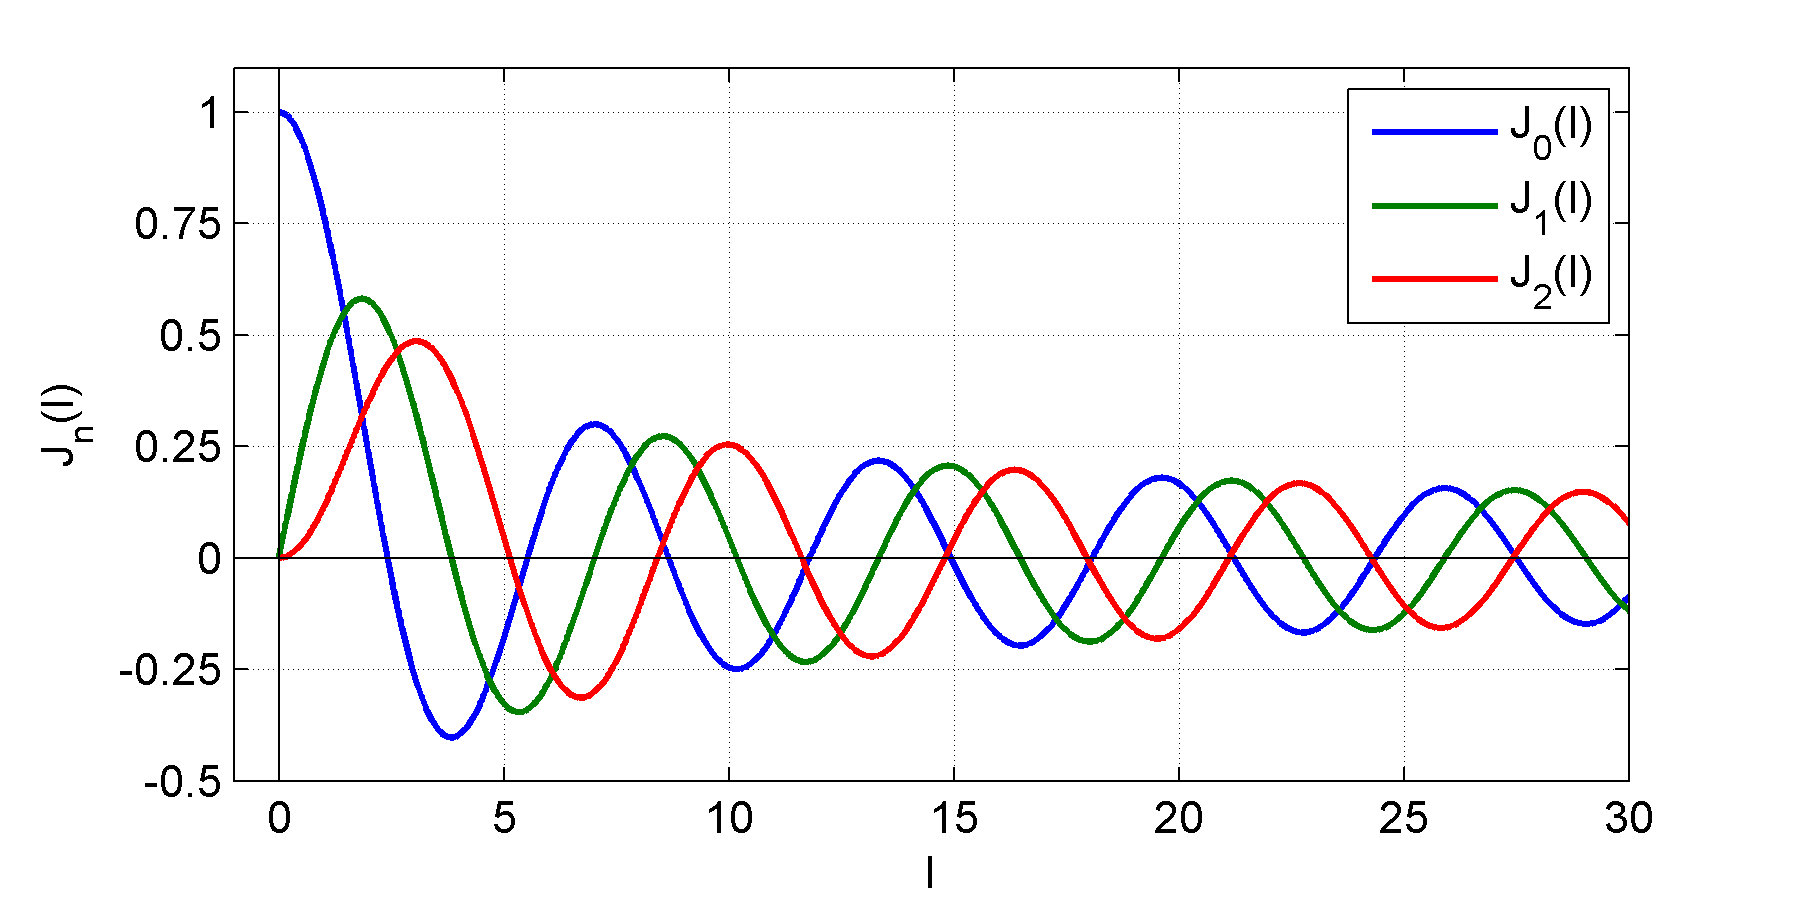
\includegraphics[width=0.80\textwidth]{Bessel2D.png}
\caption{2D-Plot der Bessel Funktionen $J_0$, $J_1$ und $J_2$.}
\label{fig:bessel2D}
\end{figure}

\FloatBarrier


Allgemein sind die Bessel-Funktionen Lösungen für die Besselsche Differentialgleichung. \cite[S. 220]{temme} Bei der FM-Synthese treten sie in Erscheinung, sobald die Formel~\ref{eq:FM_Chowning} der FM-Synthese als Fourier-Reihe dargestellt wird. Eine Fourier-Reihe setzt sich aus der Addition aus Sinus Funktionen multipliziert mit einem Fourier-Koeffizienten zusammen. Für die FM-Synthese entspricht dieser Koeffizient der Bessel-Funktionen erster Ordnung. \cite[S. 221]{lathi} Die genaue mathematische Herleitung soll an dieser Stelle nicht behandelt werden. Es soll jedoch angemerkt sein, dass $J_n(x)$ nicht elementar berechnet werden kann und numerisch bestimmt werden muss. \cite[S. 385]{abramowitz} Funktionswerte können in geeigneten Tabellen nachgeschlagen werden. \cite{davis}

Wie oben beschrieben, besteht ein Klang nicht nur aus seinem Grundton sondern auch aus Seitenfrequenzbänder. Theoretisch treten unendlich viele solcher Frequenzbänder auf, jedoch werden diese nicht mehr vom Ohr wahrgenommen, wenn sie eine gewisse Grenze an Intensität unterschreiten. \cite[S. 221]{lathi}
Die Amplitude der Trägerschwingung lässt sich durch $J_0(I)$ berechnen, wobei $I$ für den Modulationsindex steht. Dies lässt sich auch einfach aus Formel~\ref{eq:chowningAddition} entnehmen. Der erste Additionsterm $J_0(I)\sin(\omega_c t)$ entspricht der Trägerfrequenz. Bei einem Modulationsindex von $I=0$ findet keine Frequenzmodulation statt. An Abbildung~\ref{fig:bessel2D} wird ersichtlich, dass $J_0(0)=1$ ist. Für alle weiteren Bessel-Funktionen gilt $J_n(0)=0$, damit reduziert sich die Addition aus Formel~ \ref{eq:chowningAddition} auf die Grundschwingung $1\cdot\sin(\omega_c t)$ und deckt sich somit mit unserer Erwartung, dass keine Modulation stattfindet. Die Amplitude der n-ten Seitenschwingung berechnet sich durch $J_n(I)$ wobei $n$ für die n-te Seitenfrequenz steht. Für Oberschwingungen ist $n$ immer positiv, für Unterschwingungen negativ. Bei negativen $n$ Werten gilt folgender Zusammenhang: \cite[S. 223]{temme}
\begin{equation*}
J_{-n}(x)=(-1)^nJ_n(x)
\end{equation*}

Die Formel drückt aus, dass für ungerade Seitenschwingungen das Vorzeichen invertiert werden muss, bei geraden Seitenschwingungen allerdings nicht. Dies ist auch in der Summenformel~\ref{eq:chowningAddition} ersichtlich. Für ungerade $n$ Werte werden die Sinus Werte subtrahiert, bei geraden $n$ addiert. 
Dies wird offensichtlich, wenn $J_n(I)$ mit der Klammer multipliziert wird, wie in Formel~\ref{eq:FormelinchenBessel} in Kapitel~\ref{matze:simplefm}.

\label{bulli:besselModIndexZusammenahang}
Wird nun der Modulationsindex stetig erhöht, wird Energie von der Grundfrequenz auf die Seitenbänder verteilt. Dieser Vorgang wird durch den Verlauf der Bessel-Funktionen bestimmt. Dies lässt sich an Abbildung~\ref{fig:bessel2D} verdeutlichen. Wird $I$ größer, fällt die Amplitude von $J_0(I)$ ab und die restlichen Bessel-Funktionen steigen an. $J_0(I)$ durchläuft den Nullpunkt bei $\approx2,5$. Das bedeutet bei einem Modulationsindex von ungefähr $2,5$ ist der Grundton nicht im Frequenzspektrum vorhanden. Es besteht daher nur noch aus Seitenfrequenzen. In Abbildung~\ref{fig:chowningEnergieVerteilung} wird der Modulationsindex von $0$ bis $4$ inkrementiert.
Es wird ersichtlich, wie immer mehr Seitenfrequenzen entstehen und dabei die Grundfrequenz abnimmt. In Abbildung~ \ref{fig:chowningEnergieVerteilung} wird der Betrag der Amplitude dargestellt, somit wird die Grundfrequenz für $I=3$ im Vergleich zu $I=2$ wieder größer, da die Bessel-Funktion den Nullpunkt durchlaufen hat und im negativen Bereich größer wird, bis das lokale Minimum erreicht wird und der Betrag wieder bis $0$ abnimmt.

\begin{figure} [ht]
\centering
  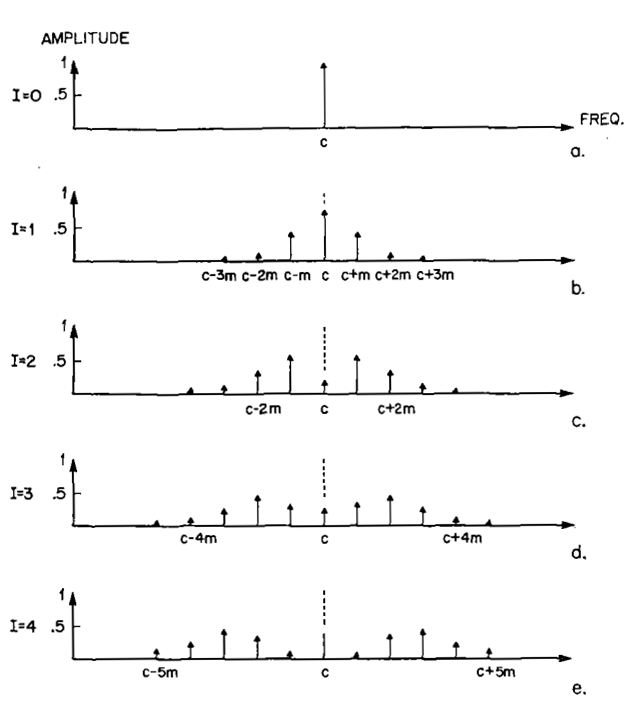
\includegraphics[width=0.5\textwidth]{Chowning_EnergieVerteilung.png}
\caption{Beispiel zur Veranschaulichung der zunehmenden Bandbreite in Abhängigkeit eines wachsenden Modulationsindex. $c$ entspricht der Trägerfrequenz; $c\pm n\cdot m$ entspricht der n-ten Seitenfrequenz.}
\label{fig:chowningEnergieVerteilung}
Quelle: \cite{chowningPaper}
\end{figure}
\FloatBarrier

An Abbildung~\ref{fig:chowningEnergieVerteilung} ist auch zu erkennen, dass die Seitenfrequenzen sich symmetrisch in negativer und positiver Richtung zur Grundfrequenz ausbreiten.
Dies wird auch an Formel~\ref{eq:chowningAddition} ersichtlich. Der innere Teil vom Sinus entspricht der Seitenfrequenz, wobei $(\omega_c+n\cdot \omega_m)$ der n-ten Oberschwingung entspricht und $(\omega_c-n\cdot \omega_m)$ der n-ten Unterschwingung. $J_n(I)$ gibt die Amplitude der n-ten Unter- und Oberschwingung an. 
Dies ist ein Vorteil der FM-Synthese im Vergleich zu anderen Sound-Synthese Verfahren. Durch eine relativ simple Änderung des Modulationsindex können komplexe Klänge mit reichem Klangspektrum erzeugt werden. Die Bandbreite $B_{FM}$ des Klangspektrums bei der FM-Synthese entspricht: \cite[S. 221]{lathi}
\begin{equation}
B_{FM}=2nf_m=2(I+1)f_m
\label{eq:fmBandwidth}
\end{equation} 
Die Bandbreite des synthetisierten Tones ist somit abhängig vom Modulationsindex und der Modulationsfrequenz. 
Dieser Zusammenhang lässt sich aus dem graphischen Verlauf der Bessel-Funktionen mit einem variablen Wert $n$ ablesen (s. \ref{fig:besselVonN}). Für einen festen Wert $I$, nimmt $J_n(I)$ ab. Für ein ausreichend großes $n$ können weitere Seitenfrequenz ignoriert werden, da ihre Amplituden vernachlässigbar klein werden. 
Durch die obige Formel kann auch ein Zusammenhang zwischen Modulationsindex und Anzahl der Seitenfrequenzbänder hergestellt werden. Die Anzahl der signifikanten Seitenfrequenzen $n$ ist in etwa $I+1$. Wird ein zeitabhängiger Modulationsindex $I(t)$ verwendet, kann die Bandbreite des Spektrums zusätzlich variiert werden. Dies schafft weitere Möglichkeiten bei der Klanggestaltung. 

\begin{figure} [ht]
\centering
  \includegraphics[width=0.75\textwidth]{BesselVonN.png}
\caption{Bessel-Funktionen in Abhängigkeit von $n$ für $I=6$. Am Verlauf der Kurve ist ersichtlich, dass die Amplituden der Seitenfrequenzen ab $n=7$ so gut wie nicht mehr vorhanden sind.}
\label{fig:besselVonN}
\end{figure}
\FloatBarrier


Wie in Kapitel \glqq \ref{PrinzipFM} \nameref{PrinzipFM}\grqq{} beschrieben, ist es jedoch schwer das Ergebnis der FM-Synthese vorherzusehen. Dies liegt zum Einen an dem schwingenden Verlauf der Bessel-Funktionen und deren Wirken auf die Seitenschwingungen. Abbildung~\ref{fig:bessel3D} stellt die Bessel-Funktionen $J_0$ bis $J_{15}$ dreidimensional, in Abhängigkeit des Modulationsindexes dar.
Durch genaue Betrachtung des Funktionsverlaufs lässt sich ein Gefühl für die Veränderung der Seitenfrequenzen entwickeln.

\begin{figure} [ht]
\centering
  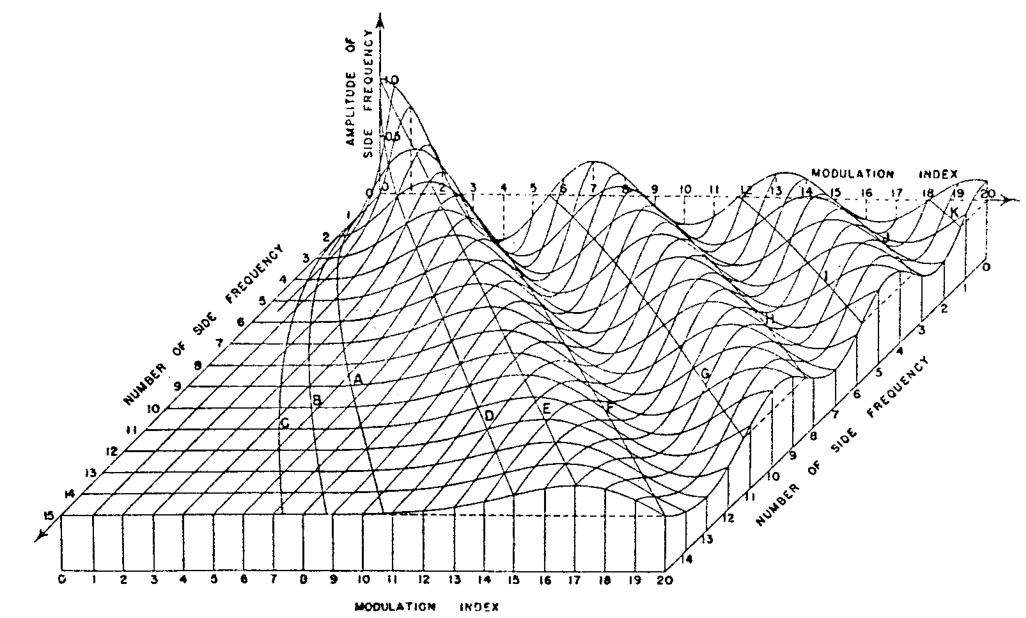
\includegraphics[width=0.90\textwidth]{ChowningBessel.png}
\caption{3D Darstellung der Bessel-Funktionen $J_0$ bis $J_{15}$ und Modulationsindex $I$ von 0 bis 20. }
\label{fig:bessel3D}
Quelle: \cite{chowningPaper}
\end{figure}
\FloatBarrier

Zwei weitere Effekte erschweren die Vorhersehbarkeit. Der erste Effekt betrifft negative Seitenfrequenzen. Eine negative Frequenz entspricht einer Phasenverschiebung von $\pi$. Daher muss das Vorzeichen der Amplitude einer solchen Frequenz invertiert werden und der Betrag der Frequenz wird verwendet. Dies lässt sich anschaulich als Punktspiegelung am Ursprung vorstellen. Chowning bezeichnet diesen Umstand als Reflexion der Frequenzen. Der zweite Effekt betrifft Frequenzen, die den selben Zahlenwert haben. Dabei werden die Amplituden der gleichen Frequenzen algebraisch addiert. Dies kann auch zuvor reflektierte Frequenzen betreffen. Daher kann es unter Umständen schwer sein, einen gegebenen Klang durch FM-Synthese zu rekonstruieren, da keine direkte Kontrolle über die Teiltöne, wie bei der additiven Synthese, gegeben ist. Abbildung~\ref{fig:chowningFreqReflektion} veranschaulicht das Verhalten der Seitenfrequenzen.

\begin{figure} [ht]
\centering
  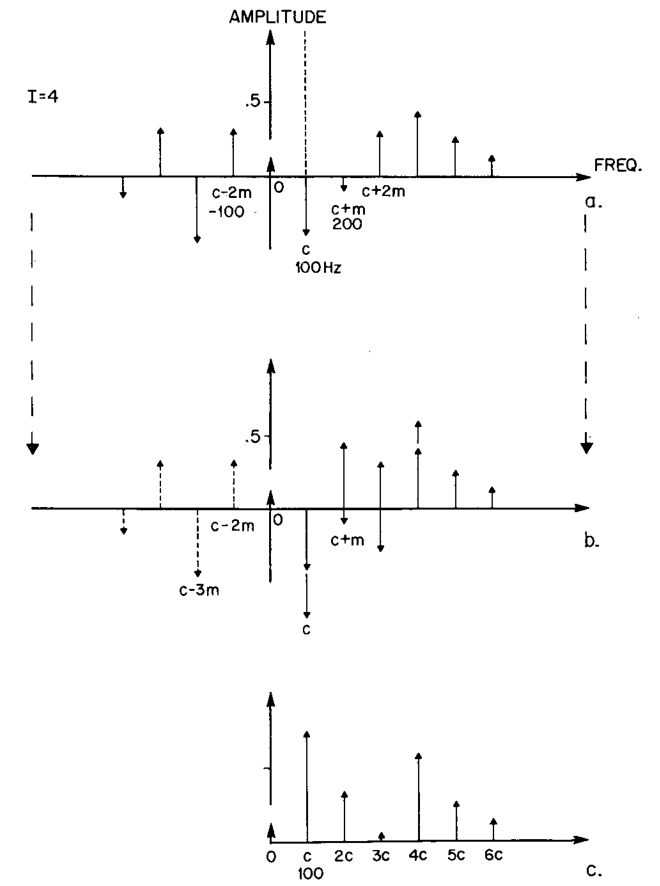
\includegraphics[width=0.5\textwidth]{ChowningFreqReflektion.png}
\caption{In \textit{a} sind alle Frequenzen an ihren ursprünglichen Positionen eingezeichnet. In \textit{b} wurden negative Frequenzen in den positiven Frequenzbereich reflektiert. \textit{c} entspricht dem endgültigen Spektrum. Für $f_c=f_m=100$ und $I=4$.}
\label{fig:chowningFreqReflektion}
Quelle: \cite{chowningPaper}
\end{figure}
\FloatBarrier




\FloatBarrier
\subsubsection{Harmonische Frequenzverhältnisse}
Bisher wurde nur wenig auf die beiden Frequenzparameter eingegangen. Diese können theoretisch beliebige Werte annehmen, so lange sie innerhalb des hörbaren Frequenzbereichs liegen. Ist das Ziel jedoch harmonische Klänge für Musik zu synthetisieren, müssen Trägerfrequenz und Modulationsfrequenz in einem besonderen Verhältnis stehen. Genauer gesagt muss das Verhältnis durch eine rationale Zahl beschrieben werden können, also durch einen Bruch aus zwei ganzen Zahlen $N_1$ und $N_2$. Somit gilt:
\begin{equation*}
\frac{f_c}{f_m}=\frac{N_1}{N_2}
\end{equation*}
Ist der Bruch $N_1/N_2$ zusätzlich gekürzt, ergibt sich für die Grundfrequenz $f_0$ der modulierten Schwingung folgende Gleichung:
\begin{equation*}
f_0=\frac{\omega_c}{N_1}=\frac{\omega_m}{N_2}
\end{equation*}
Für die Positionen der Seitenfrequenzen in der harmonischen Reihe des Klangs gilt:
\begin{align}
k=N_1+n\cdot N_2
\end{align}
Wobei $k$ der Nummer der Harmonischen entspricht und $n$ der n-ten Seitenfrequenz. Unter den obigen Bedingungen lassen sich weitere, für die Klangerzeugung hilfreiche Aussagen treffen: \cite{chowningPaper}
\begin{lstlisting}[mathescape]
1) Die Trägerfrequenz ist immer die $N_1$-te Harmonische.
2) Für $N_2=1$ enthält das Spektrum alle Harmonischen und der Grundton entspricht der Modulationsfrequenz.
3) Wenn $N_2$ gerade ist, enthält das Spektrum nur ungerade Harmonische.
4) Ist $N_2=3$, fehlt jede dritte Harmonische in der Reihe der Harmonischen.
\end{lstlisting}
Die tatsächliche Anzahl der Harmonischen im modulierten Signal mit ausreichend großer Amplitude ist abhängig vom Modulationsindex. Für kleine Indizes und Frequenzverhältnisse mit $N_1\neq1$ kann der Grundton nicht im erzeugten Klang vorhanden sein. Die Seitenschwingungen im negativen Frequenzbereich werden, wie weiter oben beschrieben, am Ursprung ins Positive gespiegelt. Solang das Verhältnis eine rationale Zahl ist, werden diese Frequenzen genau auf die positiven Frequenzen der Harmonischen reflektiert und auf diese addiert.
Es entstehen somit keine neuen Frequenzen neben den Harmonischen. Ist das Verhältnis der beiden Frequenzen jedoch irrational, 
zum Beispiel $f_c/f_m=1/\sqrt{2}$, treffen die reflektierten Frequenzen nicht genau auf die positiven Frequenzen und erzeugen somit Seitenfrequenzen, die kein ganzzahlig Vielfaches der Grundfrequenz sind. Es resultiert ein disharmonisches Klangspektrum.

Ein weiteres, erwähnenswertes Frequenzverhältnis tritt auf, wenn die Modulationsfrequenz relativ gering ist.
Wie in \glqq \ref{geschichteFMSynthese} \nameref{geschichteFMSynthese}\grqq{} beschrieben, entdeckte Chowning nach eigener Angabe die FM-Synthese beim Experimentieren mit einem Vibrato. Der Begriff Vibrato kommt aus der Musik und beschreibt eine oszillierende, leichte Variation der Tonhöhe und somit der Frequenz. Dieser Effekt ist gerade bei Violinisten erwünscht und lässt den Ton "'reicher"' und "'zarter"' klingen. \cite[S. 422]{tobias} Da der Vibrato eine Abweichung der Tonhöhe und somit eine periodische Änderung der Frequenz ist, lässt sich einfach nachvollziehen wie Chowning beim Experimentieren mit verschiedenen Zahlenwerten die FM-Synthese entdeckte. Von einem Vibrato wird gesprochen, wenn die Modulationsfrequenz unter 20 Hz liegt. In Abbildung~\ref{fig:vibrato} ist ein Vibrato in einem Spektrogramm dargestellt, die oszillierende Trägerfrequenz lässt sich gut erkennen.

Die beschriebenen Zusammenhänge zwischen Träger- und Modulationsfrequenz stellen interessante Eigenschaften der FM-Synthese dar. Sie können einen praktischen Mehrwert bringen bei der Nachbildung von Tönen. So kann zum Beispiel gezielt ein harmonisches Klangspektrum erzeugt werden oder eben nicht, je nachdem welches Instrument rekonstruiert werden soll.

\begin{figure} [ht]
\centering
  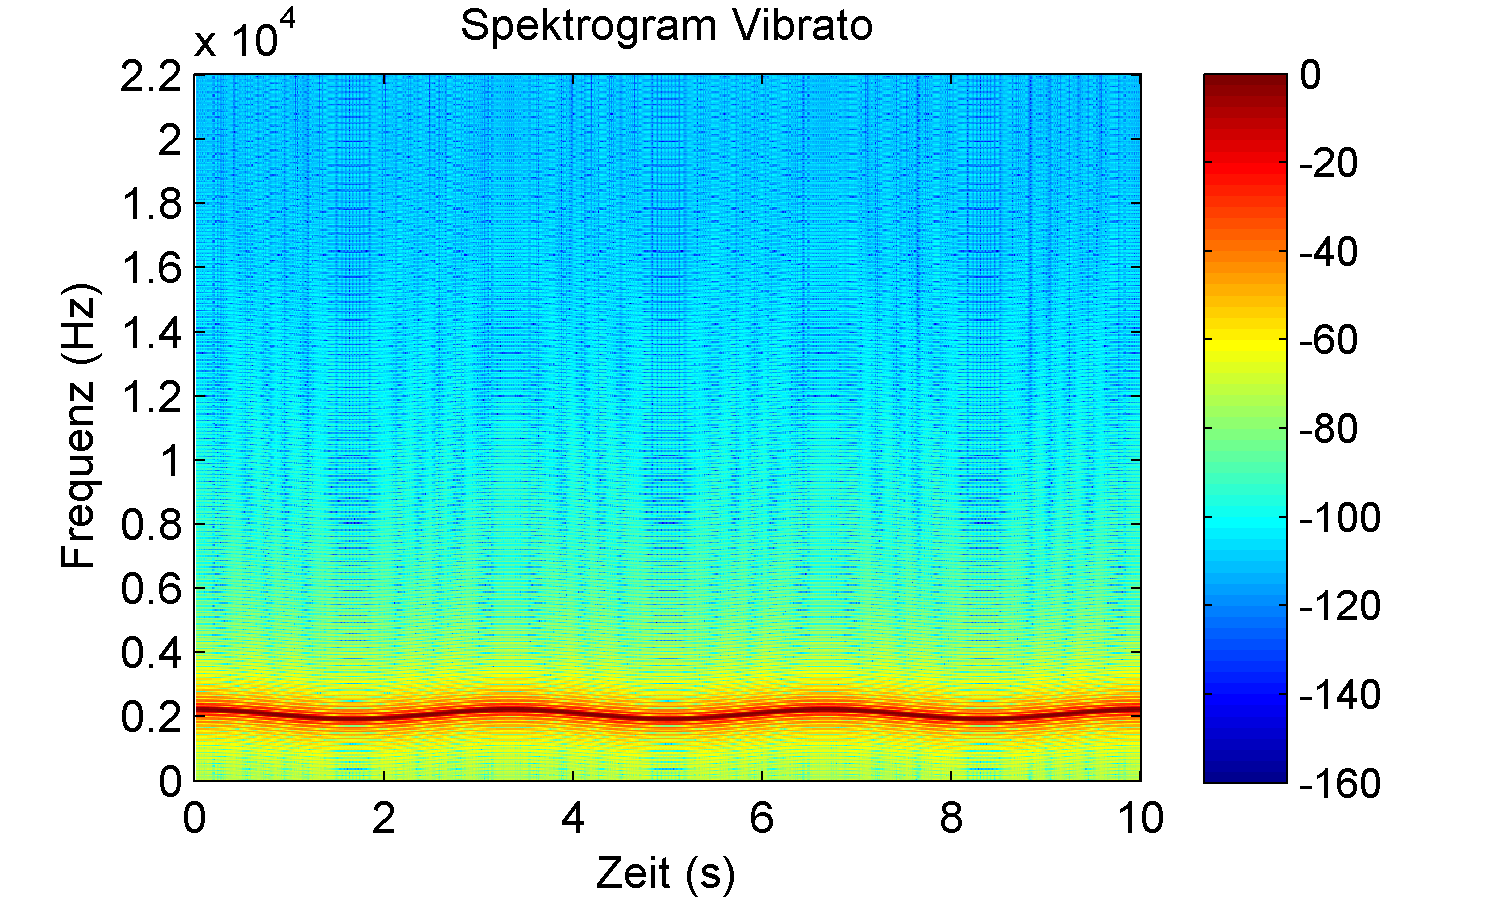
\includegraphics[width=0.60\textwidth]{vibrato.png}
\caption{Gut sichtbarer Vibrato bei einer Trägerfrequenz von 2093 Hz, was einem C4 Ton entspricht. Die Modulationsfrequenz ist mit 0.3 Hz sehr niedrig gewählt und der Modulationsindex relativ hoch mit $I=500$.}
\label{fig:vibrato}
\end{figure}




\FloatBarrier 